\documentclass[10.5pt]{beamer}
\usetheme{CambridgeUS}
\usepackage{amsmath, amssymb}
\usepackage{mathrsfs}
\usepackage{listings}
\usepackage{cite}
\usepackage{bm}
\setbeamertemplate{caption}[numbered]
\usepackage{tikz}
\usetikzlibrary{arrows.meta}
\usetikzlibrary{positioning,arrows.meta}
\usetikzlibrary{arrows.meta, positioning, shapes.geometric, calc}
\usecolortheme{beaver}

\setbeamertemplate{footline}
{
  \leavevmode%
  \hbox{%
    \begin{beamercolorbox}[wd=0.25\paperwidth,ht=2.5ex,dp=1ex,left]{author in head/foot}%
      \usebeamerfont{author in head/foot}\hspace*{1em}\insertshortauthor
    \end{beamercolorbox}%
    \begin{beamercolorbox}[wd=0.6\paperwidth,ht=2.5ex,dp=1ex,center]{title in head/foot}%
      \usebeamerfont{title in head/foot}\insertshorttitle
    \end{beamercolorbox}%
    \begin{beamercolorbox}[wd=0.08\paperwidth,ht=2.5ex,dp=1ex,right]{date in head/foot}%
       \insertframenumber{} / \inserttotalframenumber\hspace*{1.5ex}
    \end{beamercolorbox}%
  }\vskip0pt%
}

\title[Radar Signal Processing]{\large{Implementation and Evaluation of Wind Profile Estimation Algorithms}}
\author[]{
\texorpdfstring{
    Naveen C Lal (20323079) \\
    Roopesh O R (20323085)\\
    Sneha S (20323094)\\
    \vspace{0.2in}
    B.Tech Electronics and Communication Engineering
    \\ SOE, CUSAT
}{Naveen C Lal (203230**), Roopesh O R (20323085), Sneha S (20323094), B.Tech Electronics and Communication Engineering, SOE, CUSAT}}
\date{November 2, 2026}
% \setcounter{tocdepth}{1}


\begin{document}
\begin{frame}
  \titlepage
\end{frame}
\begin{frame}{Project Overview }
Project Guide: Dr Binu Paul \\
Project Phase: Phase 1\\
Research Area: Radar Signal Processing\\
Focus: Evaluation and comparison of MCCF, IME and hybrid method\\

\end{frame}

%--- Outline ---
\begin{frame}{Presentation Outline}
\small
    \tableofcontents
\end{frame}

%----------- Introduction -----------
\section{Introduction}

\subsection{Introduction to Wind Profiler Radar}
\begin{frame}{Introduction to Wind Profiler Radar}
\begin{columns}[T]
\begin{column}{.58\textwidth}
\begin{itemize}
    \item Wind profiler radars use electromagnetic waves to estimate atmospheric wind profiles remotely.
    \item The Doppler shift of returned atmospheric echoes
    provides information about radial wind velocity.
    \item Doppler power spectra are used to estimate important parameters:
    \begin{itemize}
        \item $M_0$ -- Signal power
        \item $M_1$ -- Mean Doppler velocity
        \item $M_2$ -- Spectral width
    \end{itemize}
    \item This project focuses on the \textbf{205 MHz ST radar at CUSAT}
\end{itemize}
\end{column}%
\hfill%
\begin{column}{.4\textwidth}
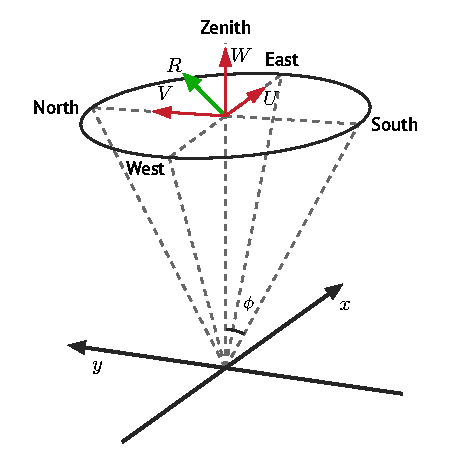
\includegraphics[width=\linewidth]{dbs.pdf}
\end{column}%
\end{columns}
\end{frame}

\subsection{Existing Problem}
\begin{frame}{Existing Problem}
\begin{itemize}
    \item Wind velocity estimation using the 205 MHz ST radar at CUSAT requires accurate identification of peaks in Doppler spectra.

    \item \textbf{Major challenges:}
    \begin{itemize}
        \item Low signal-to-noise ratio (SNR)
        \item Ground clutter and unwanted interference
        \item Multiple spectral peaks and ambiguous peak selection
    \end{itemize}

    \item Incorrect peak detection leads to errors in Doppler velocity
    estimation and discontinuities in wind profiles.

    \item \textbf{Objective:} Compare MCCF, IME, and hybrid methods
    to study their accuracy under different radar signal conditions.
\end{itemize}
\end{frame}

\subsection{Project Overview}
\begin{frame}{Project Overview}
\begin{block}{Research Focus}
Reliable Doppler spectral peak and moment estimation
for the 205 MHz ST radar at CUSAT.
\end{block}

\vspace{0.15cm}

\textbf{Methods Investigated}
\begin{itemize}
    \item \textbf{MCCF:} Mutual Convolution Cost Function
    \item \textbf{IME:} Improved Moments Estimation
    \item \textbf{Hybrid Methods:} Combining mutual convolution with IME processing (Hybrid 1 and Hybrid 2)
\end{itemize}

\vspace{0.15cm}

\textbf{Main Objective}
\begin{itemize}
    \item Evaluate the methods on radar spectra.
    \item Evaluate performance using synthetic data with known parameters.
\end{itemize}

\end{frame}
\subsection{project workflow}
\begin{frame}{Project Workflow}
    \centering
    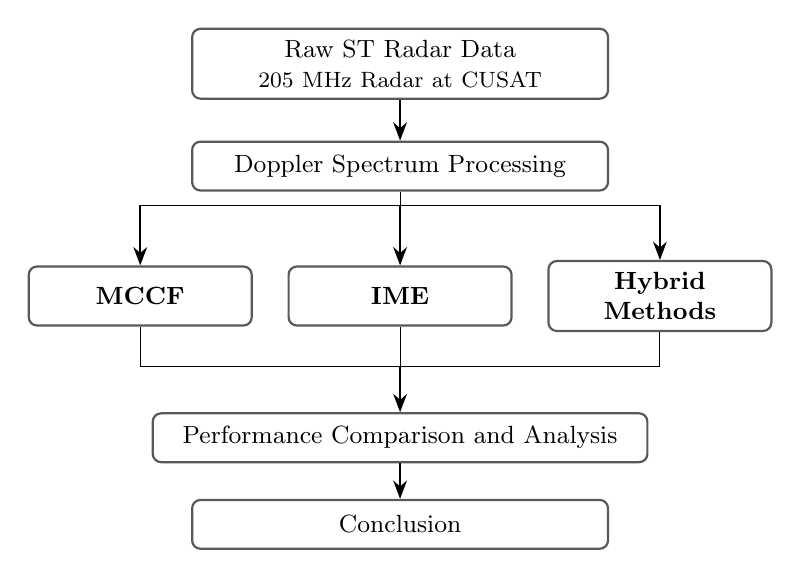
\begin{tikzpicture}[
    >=Stealth,
    block/.style={
        rectangle, rounded corners=3pt,
        draw=black!65, thick,
        align=center,
        text width=5.0cm,
        minimum height=0.62cm,
        inner sep=4pt,
        font=\small
    },
    method/.style={
        rectangle, rounded corners=3pt,
        draw=black!65, thick,
        align=center,
        text width=2.55cm,
        minimum height=0.75cm,
        inner sep=4pt,
        font=\small
    },
    arrow/.style={->, thick}
]

% Main input
\node[block] (raw) at (0,0)
{Raw ST Radar Data\\
\footnotesize 205 MHz Radar at CUSAT};

\node[block] (spectrum) at (0,-1.3)
{Doppler Spectrum Processing};

% Parallel algorithms
\node[method] (mccf) at (-3.3,-2.95)
{\textbf{MCCF}};

\node[method] (ime) at (0,-2.95)
{\textbf{IME}};

\node[method] (hybrid) at (3.3,-2.95)
{\textbf{Hybrid Methods}};

% Evaluation and conclusion
\node[block, text width=6.0cm] (eval) at (0,-4.75)
{Performance Comparison and Analysis};

\node[block] (conclusion) at (0,-5.85)
{Conclusion};

% Input arrows
\draw[arrow] (raw.south) -- (spectrum.north);

% Branch to all three methods
\coordinate (split) at (0,-1.8);

\draw (spectrum.south) -- (split);
\draw (split) -- (-3.3,-1.8);
\draw (split) -- (3.3,-1.8);

\draw[arrow] (-3.3,-1.8) -- (mccf.north);
\draw[arrow] (0,-1.8) -- (ime.north);
\draw[arrow] (3.3,-1.8) -- (hybrid.north);

% Merge the outputs below all method boxes
\coordinate (merge) at (0,-3.85);

\draw (mccf.south) -- (-3.3,-3.85);
\draw (ime.south) -- (0,-3.85);
\draw (hybrid.south) -- (3.3,-3.85);

\draw (-3.3,-3.85) -- (3.3,-3.85);
\draw[arrow] (merge) -- (eval.north);

% Final stage
\draw[arrow] (eval.south) -- (conclusion.north);

\end{tikzpicture}
\end{frame}

\section{Algorithms}

\subsection{MCCF}
\begin{frame}{MCCF: Working Principle}
\begin{itemize}
    \item A Doppler spectral peak estimation method with noise suppression.

    \vspace{0.2cm}

    \item {Processing Stages}
    \begin{itemize}
        \item \textbf{Preprocessing:} FFT and DC-component removal.
        \item \textbf{Noise Suppression:} Mutual convolution and MCLMS adaptive filtering.
        \item \textbf{Peak Selection:} Candidate peaks are evaluated using a velocity-continuity and magnitude-based cost function.
        \item \textbf{Moment Estimation:} Estimate the Doppler spectral moments from the selected peak.
    \end{itemize}

    \vspace{0.2cm}

    \item Improve spectral quality and select a suitable peak instead of relying only on the strongest spectral component.

\end{itemize}
\end{frame}
\begin{frame}{MCCF: Algorithm Flow}
    \centering
    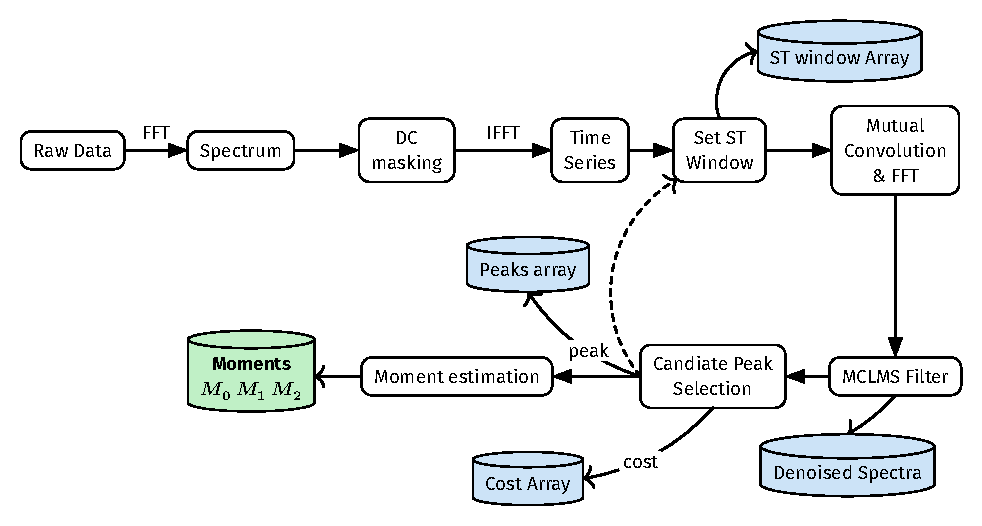
\includegraphics[width=0.9\linewidth]{mccf.pdf}
\end{frame}

\begin{frame}{MCCF: Important steps}
\begin{itemize}
    \item \textbf{Setting Space-Time window}: Limits peak search window to a selected Doppler range (space). (No time window is used due to the large time difference between observations)
    \item \textbf{Mutual Convolution}: Divides the single spectrum into slices of half length and convolves them together to generate multiple intermediate combined results.
    Pick the result with the highest peak
    \item \textbf{Modified Complex Least Mean Square Filter}: Isolate the stable, coherent features and remove random noise and ground clutter that fluctuate unpredictably across different delay steps
\end{itemize}
    
\end{frame}

\begin{frame}{MCCF: Results and Observations}
\begin{figure}
\centering
\begin{minipage}{0.32\textwidth}
    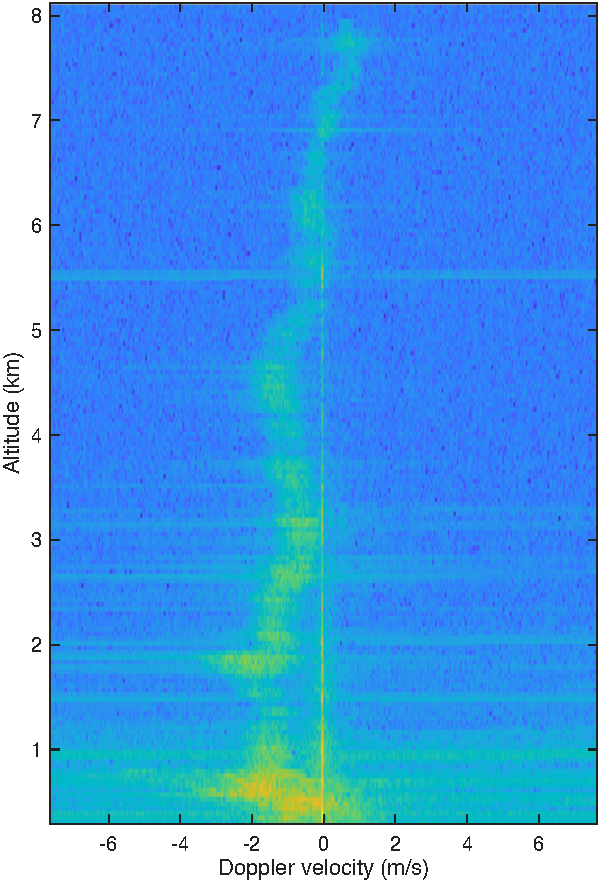
\includegraphics[height=0.62\textheight]{mccf-raw.pdf}
    \caption{\scriptsize Original Spectrum}
\end{minipage}
\hfill
\begin{minipage}{0.34\textwidth}
    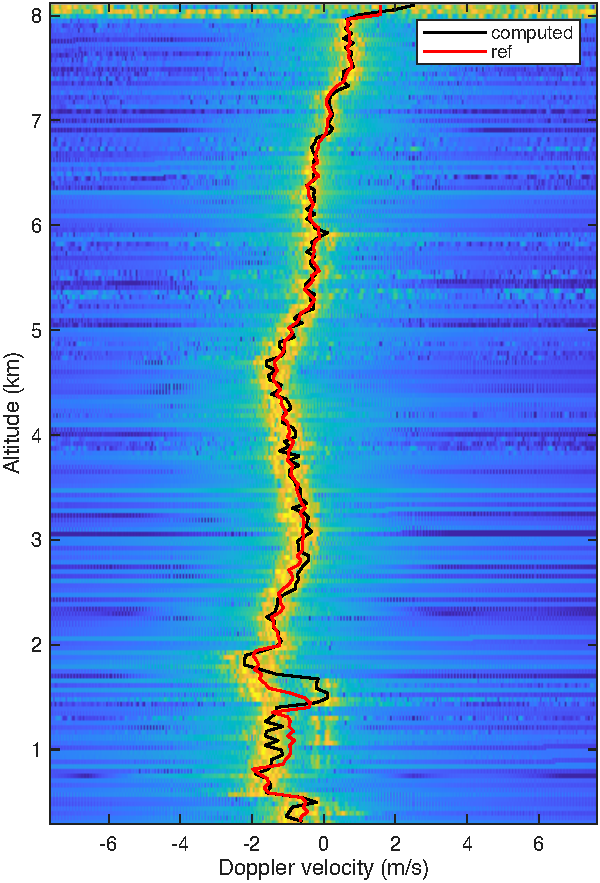
\includegraphics[height=0.62\textheight]{mccf-dspec.pdf}
    \caption{\scriptsize Estimated Moments}
\end{minipage}
\hfill
\begin{minipage}{0.32\textwidth}
    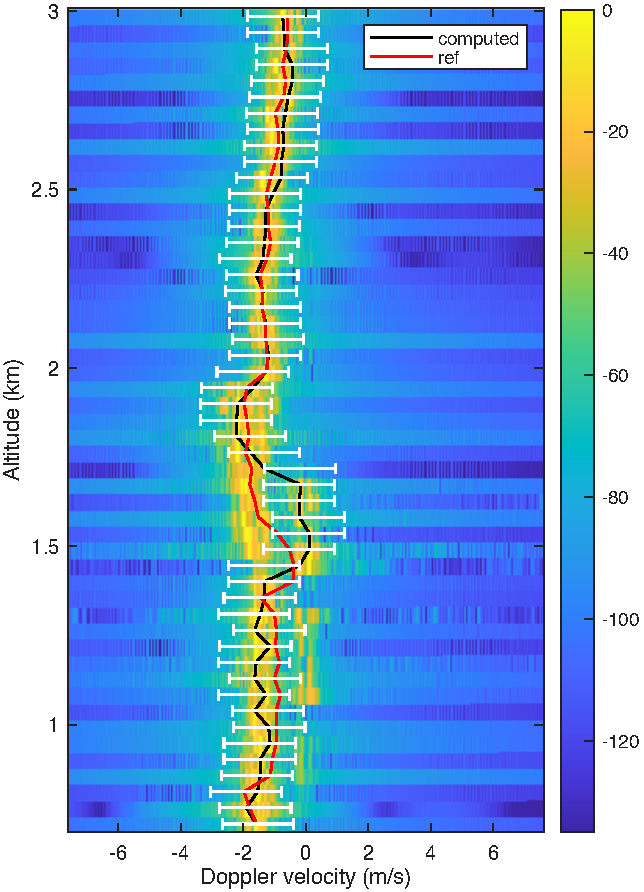
\includegraphics[height=0.62\textheight]{mccf-stw.pdf}
    \caption{\scriptsize ST window}
\end{minipage}
\end{figure}
\end{frame}

\subsection{IME}
\begin{frame}{IME: Working Principle}
\begin{block}{}
A Doppler spectral estimation method designed to identify
reliable atmospheric peaks under noisy and low-SNR conditions.
\end{block}

\vspace{0.15cm}
\textbf{Main Processing Stages}
\begin{itemize}
    \item {Spectral Preprocessing}
    \begin{itemize}
        \item Remove DC components and ground clutter.
        \item Apply 5-point smoothing and estimate the noise level.
    \end{itemize}

    \vspace{0.15cm}

    \item {Adaptive Doppler Window}
    \begin{itemize}
        \item Restrict peak searching to a selected Doppler range.
        \item Identify prospective peaks using their SNR.
    \end{itemize}

    \vspace{0.15cm}

    \item {Profile Tracing}
    \begin{itemize}
        \item Connect candidate peaks across adjacent range bins.
        \item Select the profile using velocity continuity and relative SNR.
    \end{itemize}
\end{itemize}

\vspace{0.1cm}

\end{frame}
% \begin{frame}{IME- Flowchart}
%     \centering
%     \resizebox{0.98\textwidth}{!}{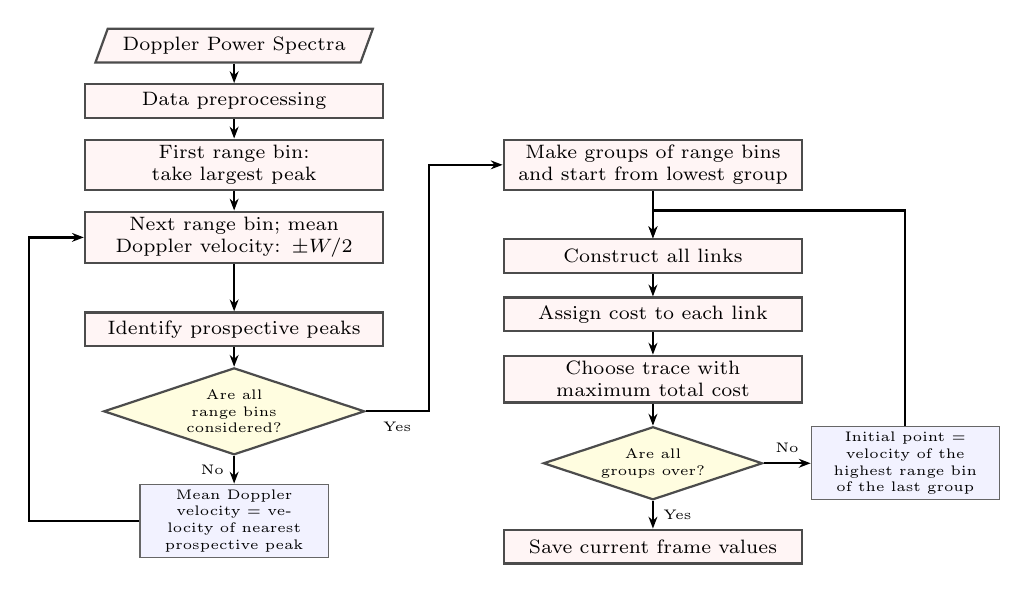
\begin{tikzpicture}[
    >=Stealth,
    process/.style={
        rectangle,
        draw=black!70,
        thick,
        fill=red!4,
        align=center,
        text width=3.65cm,
        minimum height=0.43cm,
        inner sep=2pt,
        font=\scriptsize
    },
    decision/.style={
        diamond,
        aspect=3.0,
        draw=black!70,
        thick,
        fill=yellow!12,
        align=center,
        text width=1.4cm,
        inner sep=1pt,
        font=\tiny
    },
    note/.style={
        rectangle,
        draw=black!60,
        fill=blue!5,
        align=center,
        text width=2.25cm,
        inner sep=2pt,
        font=\tiny
    },
    arrow/.style={-{Stealth[length=1.5mm]}, thick}
]

% =================================================
% LEFT: PEAK IDENTIFICATION AND RANGE-BIN PROCESSING
% =================================================

\node[
    trapezium,
    trapezium left angle=70,
    trapezium right angle=110,
    draw=black!70,
    thick,
    fill=red!4,
    align=center,
    text width=3 cm,
    inner sep=3pt,
    font=\scriptsize
] (raw) at (-2.8,5.1)
{Doppler Power Spectra};

\node[process, below= 7pt of raw] (pre)
{Data preprocessing};

\node[process, below= 7pt of pre] (init)
{First range bin: take largest peak};

\node[process, below= 7pt of init] (window)
{Next range bin; mean Doppler velocity: $\pm W/2$};

\node[process, below= 17pt of window] (peaks)
{Identify prospective peaks };

\node[decision, below= 7pt of peaks] (allbins)
{Are all range bins considered?};

\node[note, below=10pt of allbins] (mean)
{Mean Doppler velocity = velocity of nearest prospective peak};

\draw[arrow] (raw.south) -- (pre.north);
\draw[arrow] (pre.south) -- (init.north);
\draw[arrow] (init.south) -- (window.north);
\draw[arrow] (window.south) -- (peaks.north);
\draw[arrow] (peaks.south) -- (allbins.north);

\draw[arrow] (allbins.south) --
    node[left,font=\tiny] {No}
    (mean.north);
\draw[arrow] (mean.west)
    -- +(-40pt, 0pt)
    |- (window.west);

% =================================================
% RIGHT: GROUPING AND TRACE SELECTION
% =================================================

\node[process, right= 1.5cm of init] (groups)
{Make groups of range bins and start from lowest group};

\node[process, below= 17pt of groups] (links)
{Construct all links};

\node[process, below= 8pt of links] (cost)
{Assign cost to each link};

\node[process, below= 8pt of cost] (trace)
{Choose trace with maximum total cost};

\node[decision, below= 8pt of trace] (allgroups)
{Are all groups over?};

\node[process, below= 10pt of allgroups] (save)
{Save current frame values};

\node[note, right= 17pt of allgroups] (initial)
{Initial point = velocity of the highest range bin of the last group};

% All range bins? YES: begin grouping
\draw[arrow] (allbins.east)
    -- +(.8cm, 0pt) node[pos=0.5, below, font=\tiny] {Yes}
    |- (groups.west);

% Main grouping and tracing path
\draw[arrow] (groups.south) -- (links.north);
\draw[arrow] (links.south) -- (cost.north);
\draw[arrow] (cost.south) -- (trace.north);
\draw[arrow] (trace.south) -- (allgroups.north);

% All groups over? YES: save values
\draw[arrow]
    (allgroups.south) --
    node[right,font=\tiny] {Yes}
    (save.north);

% All groups over? NO: update initial point
\draw[arrow] (allgroups.east) --
    node[above,font=\tiny] {No}
    (initial.west);

% Updated initial point: construct links for next group
\draw[arrow] (initial.north)
    |- ([yshift=10pt]links.north)
    -| (links.north);

\end{tikzpicture}%}
% \end{frame}
\begin{frame}{(a): Preprocessing}
\small


\begin{itemize}
    \item \textbf{DC and Ground Clutter Removal}
    \begin{itemize}
        \item Suppress the zero-frequency component by interpolating neighbouring frequency bins.
    \end{itemize}

    \item \textbf{Smoothing and Filtering}
    \begin{itemize}
        \item Apply a five-point moving-average filter to reduce
        transient interference.
    \end{itemize}

    \item \textbf{Noise Estimation and Reduction}
    \begin{itemize}
        \item Estimate noise power using the Hildebrand--Sekhon method.
        \item Subtract the estimated noise and clip negative values to zero.
    \end{itemize}
\end{itemize}

\vspace{0.15cm}
\end{frame}
\begin{frame}{(b): Adaptive Doppler Window}
\begin{columns}[T,onlytextwidth]
\begin{column}{0.53\textwidth}
\textbf{Adaptive Window Selection}
\begin{itemize}
    \item Start from the lowest range bin.
    \item Use its maximum peak as the initial mean Doppler velocity.
    \item Centre the next Doppler window around the candidate closest to the previous mean velocity.
\end{itemize}
\vspace{0.1cm}
\textbf{Prospective Peak Selection}
\begin{itemize}
    \item Detect peaks within the adaptive window 
    \item Retain peaks with SNR $>0$ dB (upto 3 Peaks).
\end{itemize}
\end{column}

\begin{column}{0.44\textwidth}
\centering
\begin{figure}
    \centering
    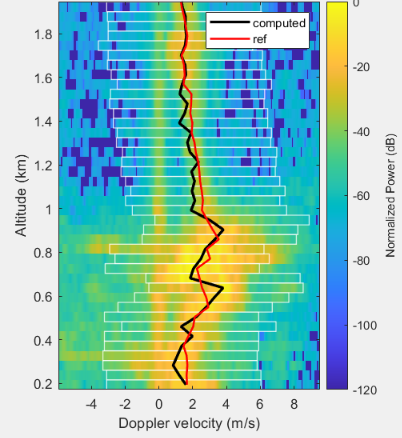
\includegraphics[width= \linewidth]{aw.png}
    \caption{Adaptive Doppler window}
\end{figure}
\end{column}
\end{columns}
\end{frame}

\begin{frame}{(c): Grouping and Cost Allocation}
\begin{columns}[T,onlytextwidth]
    \begin{column}{0.55\textwidth}
    \begin{enumerate}
        \item Grouping and Link Construction
        \item Cost Function: The link cost combines velocity continuity and normalised SNR:
        \[ C = w_1 T + w_2 P \]
        \item Final Profile Selection
        \begin{itemize}
            \item Select the trace with the maximum total cost.
            \item Use its final velocity to initialise the next group.
        \end{itemize}
    \end{enumerate}
\end{column}
\begin{column}{0.42\textwidth}
\centering
    \begin{figure}
        \centering
        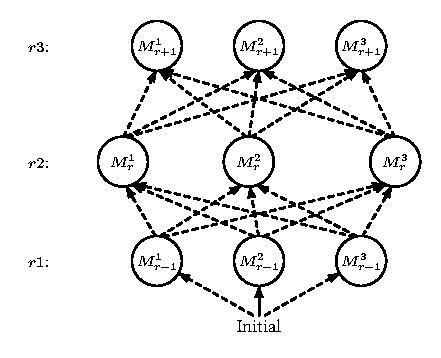
\includegraphics[width=1\linewidth]{ime-chain.pdf}
        {\caption{Grouping and profile tracing}}
    \end{figure}
\end{column}

\end{columns}
\end{frame}
\begin{frame}{IME: Results}
\begin{figure}
    \centering
    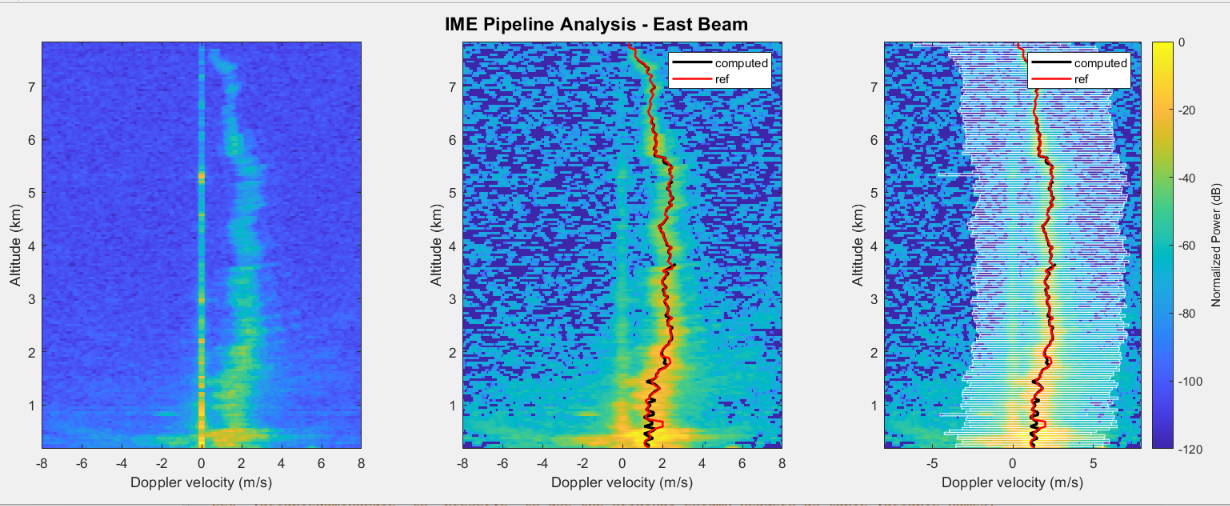
\includegraphics[width=\linewidth]{ime.png}
    \caption{a) Original     b) After applying IME    c) Adaptive window}
\end{figure}
    
\end{frame}

\subsection{Hybrid Methods}
\begin{frame}{Hybrid Methods}
\small


Mutual convolution (MC) in MCCF provides noise suppression,
while IME provides adaptive peak selection and profile tracing.
The hybrid methods combine these processing stages.


\vspace{0.35 cm}

\begin{columns}[T,onlytextwidth]

    \begin{column}{0.48\textwidth}
        \begin{block}{Hybrid 1}
            \centering
            \textbf{MC + IME Denoising + IME Peak Selection}

            \vspace{0.2cm}

            \begin{itemize}
                \item Spectrum processing using MC
                \item IME denoising
                \item IME peak selection
            \end{itemize}
        \end{block}
    \end{column}

    \begin{column}{0.48\textwidth}
        \begin{block}{Hybrid 2}
            \centering
            \textbf{MC + IME Peak Selection}

            \vspace{0.2cm}

            \begin{itemize}
                \item Spectrum processing using MC
                \item Direct IME peak selection
                % \item IME profile tracing
            \end{itemize}
        \end{block}
    \end{column}

\end{columns}

\vspace{0.2cm}
\end{frame}
\begin{frame}{Hybrid Methods: Flowchart}
\centering

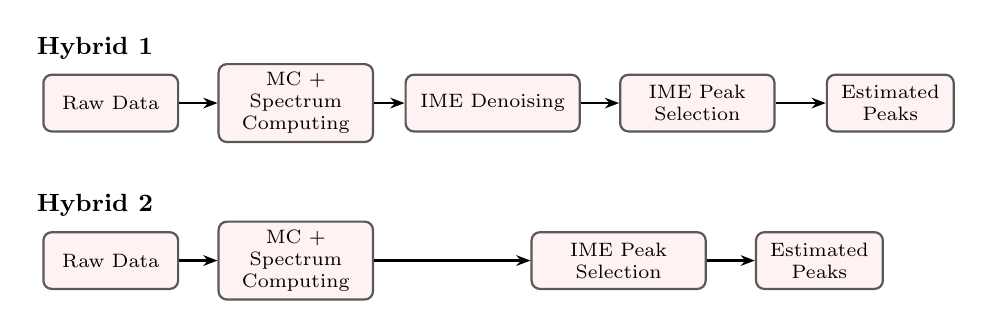
\begin{tikzpicture}[
    >=Stealth,
    block/.style={
        rectangle,
        rounded corners=3pt,
        draw=black!65,
        thick,
        fill=red!5,
        align=center,
        text width=1.75cm,
        minimum height=0.72cm,
        inner sep=3pt,
        font=\scriptsize
    },
    arrow/.style={-{Stealth[length=1.8mm]}, thick}
]

% ---------------- HYBRID 1 ----------------
\node[font=\small\bfseries] at (-5.2,1.65)
{Hybrid 1};

\node[block, text width=1.5cm] (raw1) at (-5.0,0.95)
{Raw Data};

\node[block] (mc1) at (-2.65,0.95)
{MC + Spectrum\\Computing};

\node[block, text width=2cm] (denoise) at (-0.15,0.95)
{IME Denoising};

\node[block] (peak1) at (2.45,0.95)
{IME Peak\\Selection};

\node[block, text width=1.4cm] (out1) at (4.9,0.95)
{Estimated\\Peaks};

\draw[arrow] (raw1.east) -- (mc1.west);
\draw[arrow] (mc1.east) -- (denoise.west);
\draw[arrow] (denoise.east) -- (peak1.west);
\draw[arrow] (peak1.east) -- (out1.west);

% ---------------- HYBRID 2 ----------------
\node[font=\small\bfseries] at (-5.2,-0.35)
{Hybrid 2};

\node[block, text width=1.5cm] (raw2) at (-5.0,-1.05)
{Raw Data};

\node[block] (mc2) at (-2.65,-1.05)
{MC + Spectrum\\Computing};

\node[block, text width=2.0cm] (peak2) at (1.45,-1.05)
{IME Peak Selection};

\node[block, text width=1.4cm] (out2) at (4.0,-1.05)
{Estimated\\Peaks};

\draw[arrow] (raw2.east) -- (mc2.west);
\draw[arrow] (mc2.east) -- (peak2.west);
\draw[arrow] (peak2.east) -- (out2.west);

% ---------------- KEY DIFFERENCE ---------------

\end{tikzpicture}
\end{frame}

%  \subsection{Comparison}
% \begin{frame}{Comparison and Analysis}
% \centering
% \scriptsize

% \renewcommand{\arraystretch}{1.5}

% \begin{tabular}{|p{1.35cm}|p{2.5cm}|p{2.7cm}|p{3.0cm}|}
% \hline
% \textbf{Method} &
% \textbf{Noise Suppression} &
% \textbf{Peak Selection} &
% \textbf{Key Characteristic} \\
% \hline

% MCCF &
% Mutual convolution and MCLMS filtering &
% Cost-based selection within a space-time Doppler window &
% Uses spectral strength and velocity continuity \\
% \hline

% IME &
% DC/clutter removal, smoothing and noise subtraction &
% Adaptive Doppler window and cost-based profile tracing &
% Restricts the search and connects candidate peaks across range bins \\
% \hline

% Hybrid 1 &
% Mutual convolution followed by IME denoising &
% IME peak selection and profile tracing &
% Combines both denoising stages \\
% \hline

% Hybrid 2 &
% Mutual convolution without separate IME denoising &
% IME peak selection and profile tracing &
% Avoids additional denoising that may remove weak peaks \\
% \hline

% \end{tabular}
% \end{frame}


\section{Validation}
\subsection{Synthetic Radar Data Generation}
\begin{frame}{Synthetic Radar Data Generation}

\begin{block}{}
Generated from a predefined
$UVW$ wind-velocity array by reversing the conventional
radar signal-processing pipeline to produce a raw data file.
\end{block}

\vspace{0.35cm}

\begin{center}
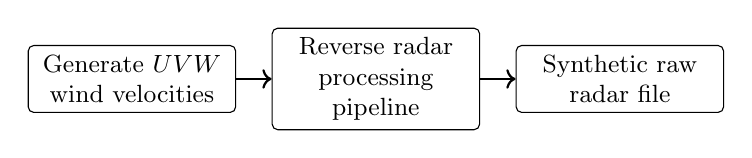
\begin{tikzpicture}[
    node distance=0.45cm,
    block/.style={
        draw,
        rectangle,
        rounded corners=2pt,
        align=center,
        minimum height=0.85cm,
        text width=2.4cm,
        font=\small
    },
    arrow/.style={->, thick}
]

\node[block] (uvw) {Generate $UVW$\\wind velocities};
\node[block, right=of uvw] (reverse) {Reverse radar\\processing pipeline};
\node[block, right=of reverse] (raw) {Synthetic raw\\radar file};

\draw[arrow] (uvw) -- (reverse);
\draw[arrow] (reverse) -- (raw);

\end{tikzpicture}
\end{center}

\vspace{0.35cm}

\begin{itemize}
    \item Provides known ground-truth wind velocities.
    \item Enables direct comparison of algorithm outputs against
    the predefined velocities.
    \item Allows controlled testing of algorithms without relying
    exclusively on newly acquired radar observations.
\end{itemize}
\end{frame}

\begin{frame}
    
\begin{figure}
    \centering
    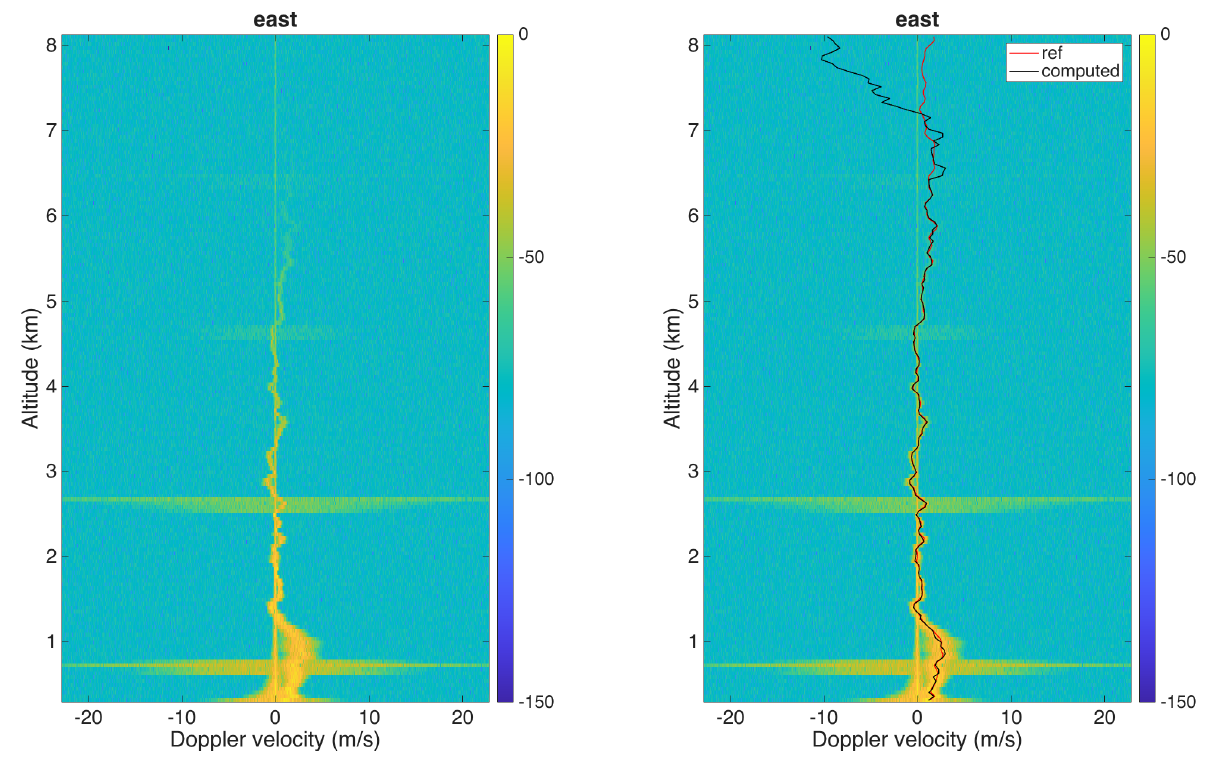
\includegraphics[width=.8\linewidth]{synth.png}
\caption{\small Synthesised raw data and corresponding velocity estimation using MCCF}
\end{figure}

\end{frame}
\section{Result}

\subsection{Evaluvation with Synthetic data}
\begin{frame}{Evaluvation with Synthetic data}
Synthesised 500 raw data samples and applied it to 5 algorithms.
\begin{columns}[T,onlytextwidth]

    % Left: MSE boxplot
    \begin{column}{0.45\textwidth}
        \centering
        \begin{figure}
            \centering
            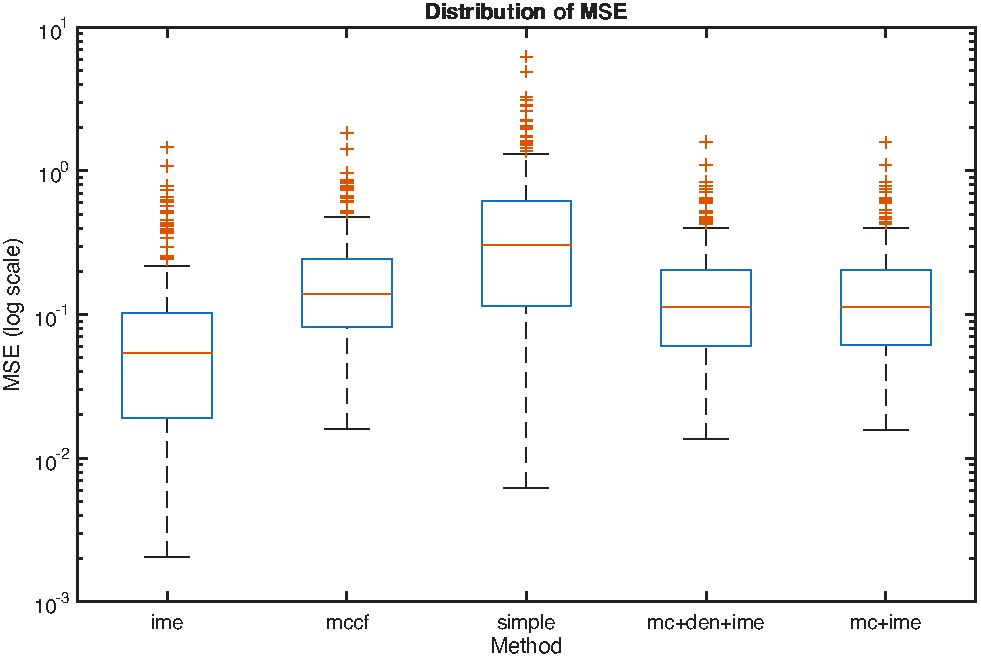
\includegraphics[width= \linewidth]{mse_distr.pdf}
            \caption{\small  Mean Squared Error (MSE)}
        \end{figure}
    \end{column}

    % Right: Correlation boxplot
    \begin{column}{0.54\textwidth}
        \centering
        \begin{figure}
            \centering
            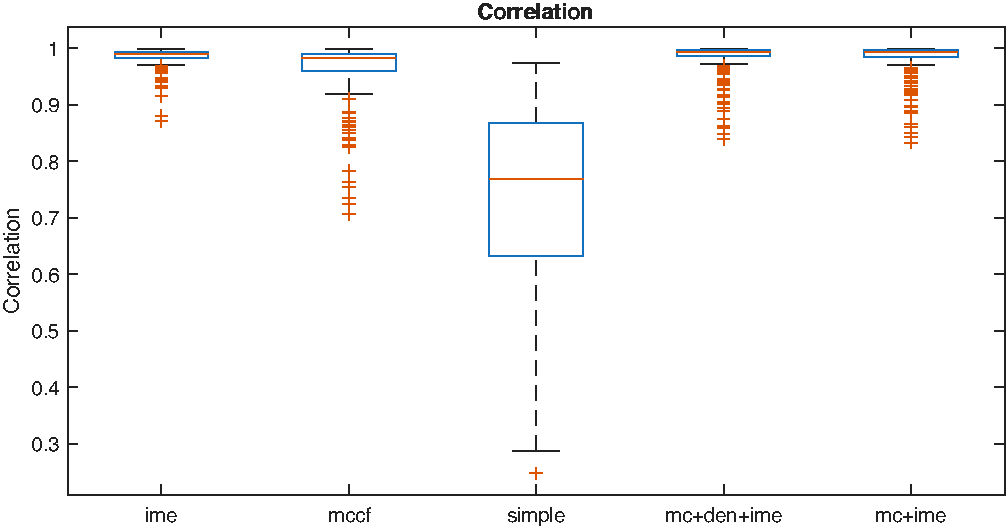
\includegraphics[width=\linewidth]{corr.pdf}
            \caption{\small  Correlation with ref data}
        \end{figure}
    \end{column}
\end{columns}
\end{frame}

\begin{frame}{Evaluvation with Synthetic data}
    \begin{figure}
        \centering
        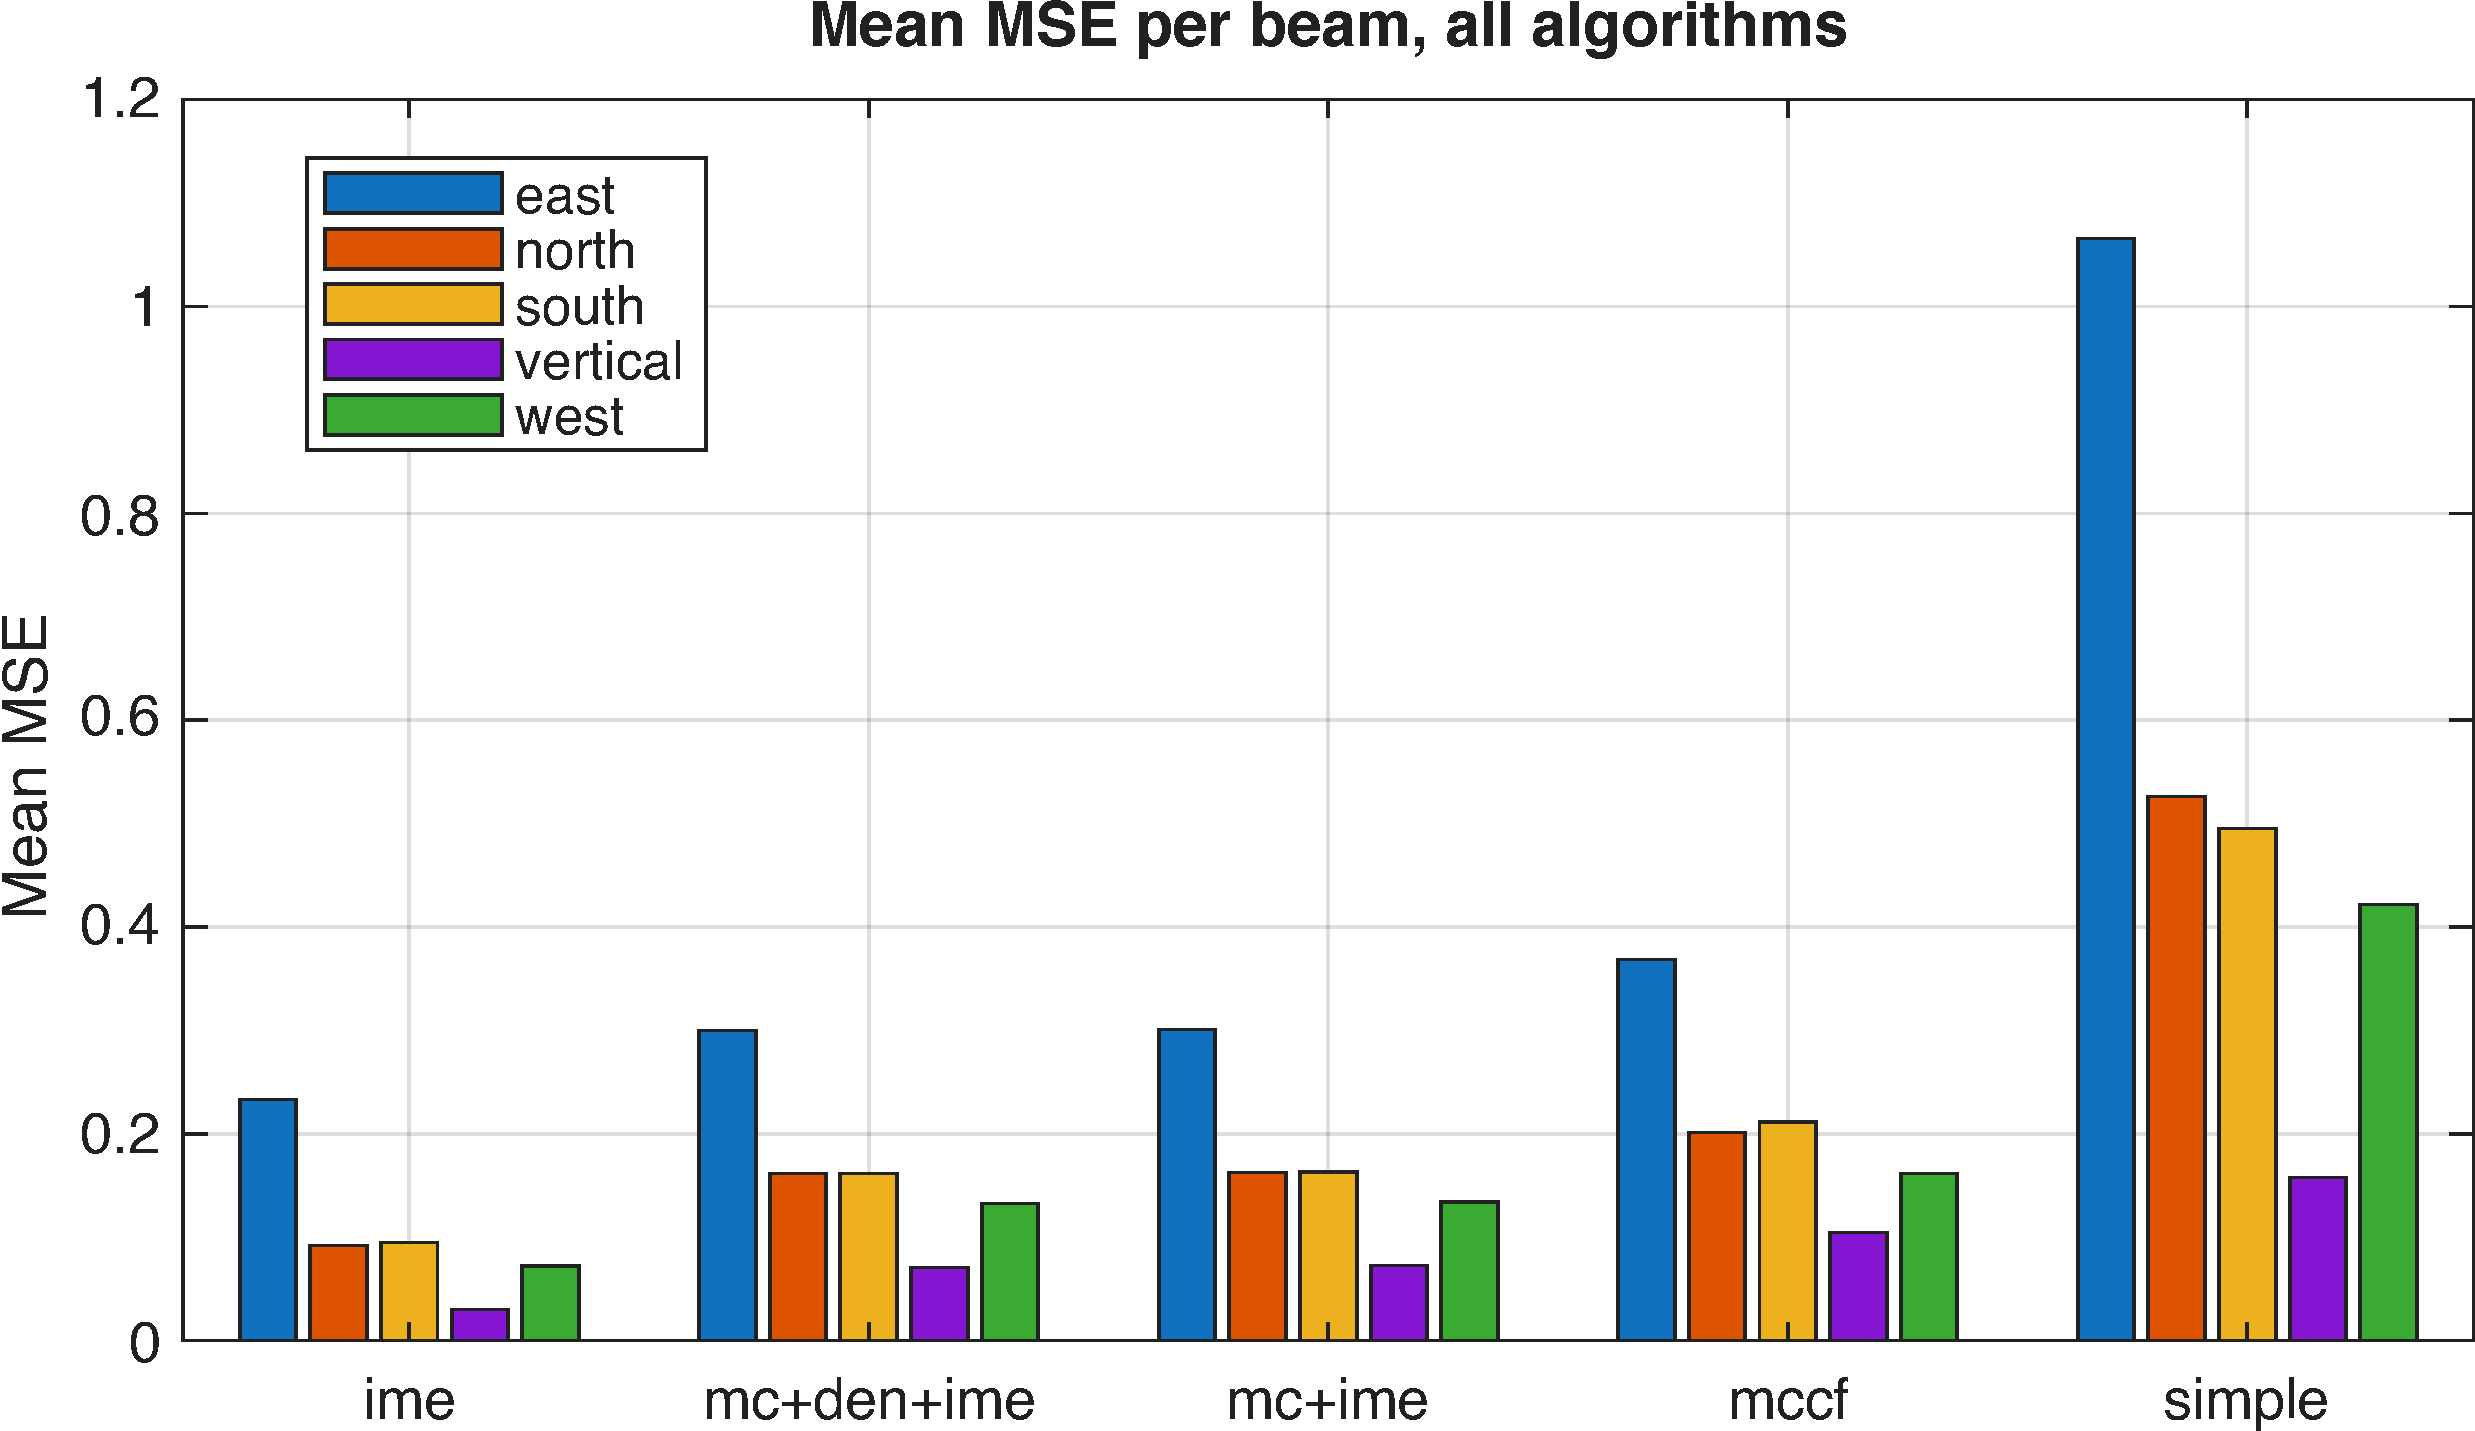
\includegraphics[width=.8\linewidth]{MSE_summary.pdf}
        \caption{MSE in all beams}
    \end{figure}
\end{frame}

\subsection{Evaluvation with Radiosonde}
\begin{frame}{Evaluvation with Radiosonde}
\begin{columns}[T, onlytextwidth]
    \begin{column}{.45\linewidth}
    \begin{itemize}
        \item Projection of radiosonde observation along with MCCF's estimation. 
        \item In the winter season, the atmosphere is stable hence, the result closely matches 
    \end{itemize}
    
    \end{column}
    \begin{column}{.5\linewidth}
    \begin{figure}
        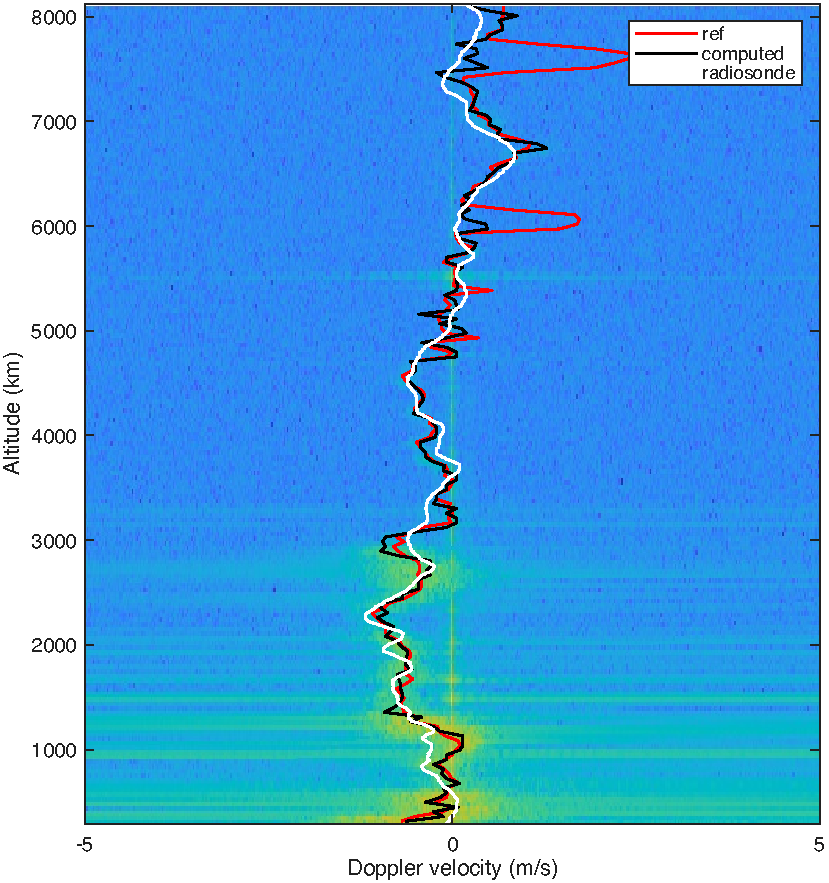
\includegraphics[width=.85\linewidth]{rs.pdf}
        \caption{Observation on 20 Jan 2026, 14:20 IST}
    \end{figure}
    \end{column}
\end{columns}
.\end{frame}

\subsection{Evaluvation with Data Pattern's output}
\begin{frame}{Evaluvation with Data Pattern's output}
Used 226 radar observations taken on 20 January 2026.

\begin{columns}[T,onlytextwidth]

    % Left: MSE boxplot
    \begin{column}{0.49\textwidth}
        \centering
        \begin{figure}
            \centering
            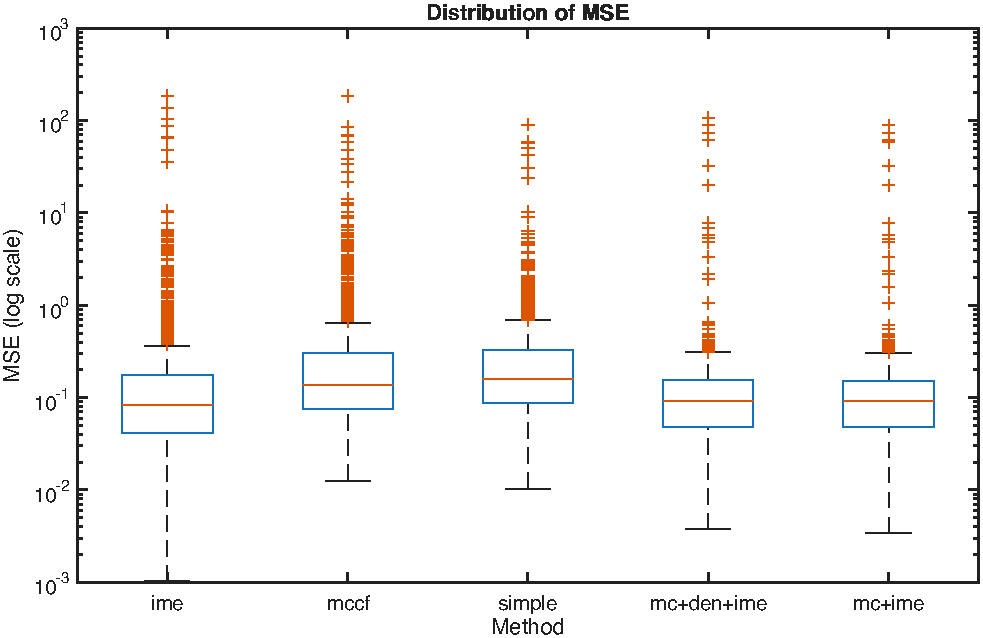
\includegraphics[width= \linewidth]{mse-distr-dp.pdf}
            \caption{\small MSE}
        \end{figure}
    \end{column}

    % Right: Correlation boxplot
    \begin{column}{0.49\textwidth}
        \centering
        \begin{figure}
            \centering
            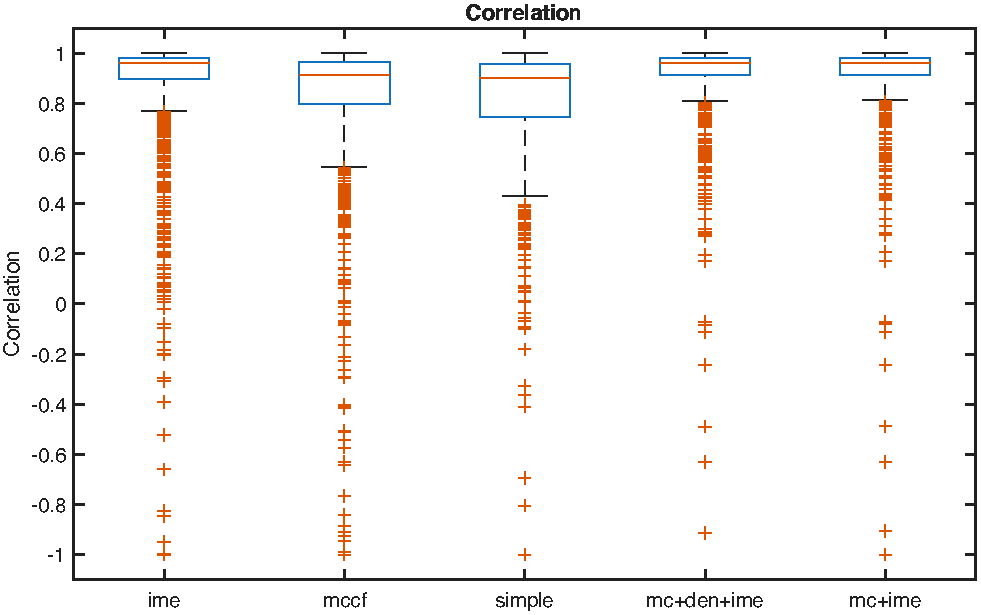
\includegraphics[width=\linewidth]{corr-dp.pdf}
            \caption{\small Correlation with reference data}
        \end{figure}
    \end{column}
\end{columns}
\end{frame}

\begin{frame}{Evaluvation with Data Pattern's output}
\begin{figure}
    \centering
    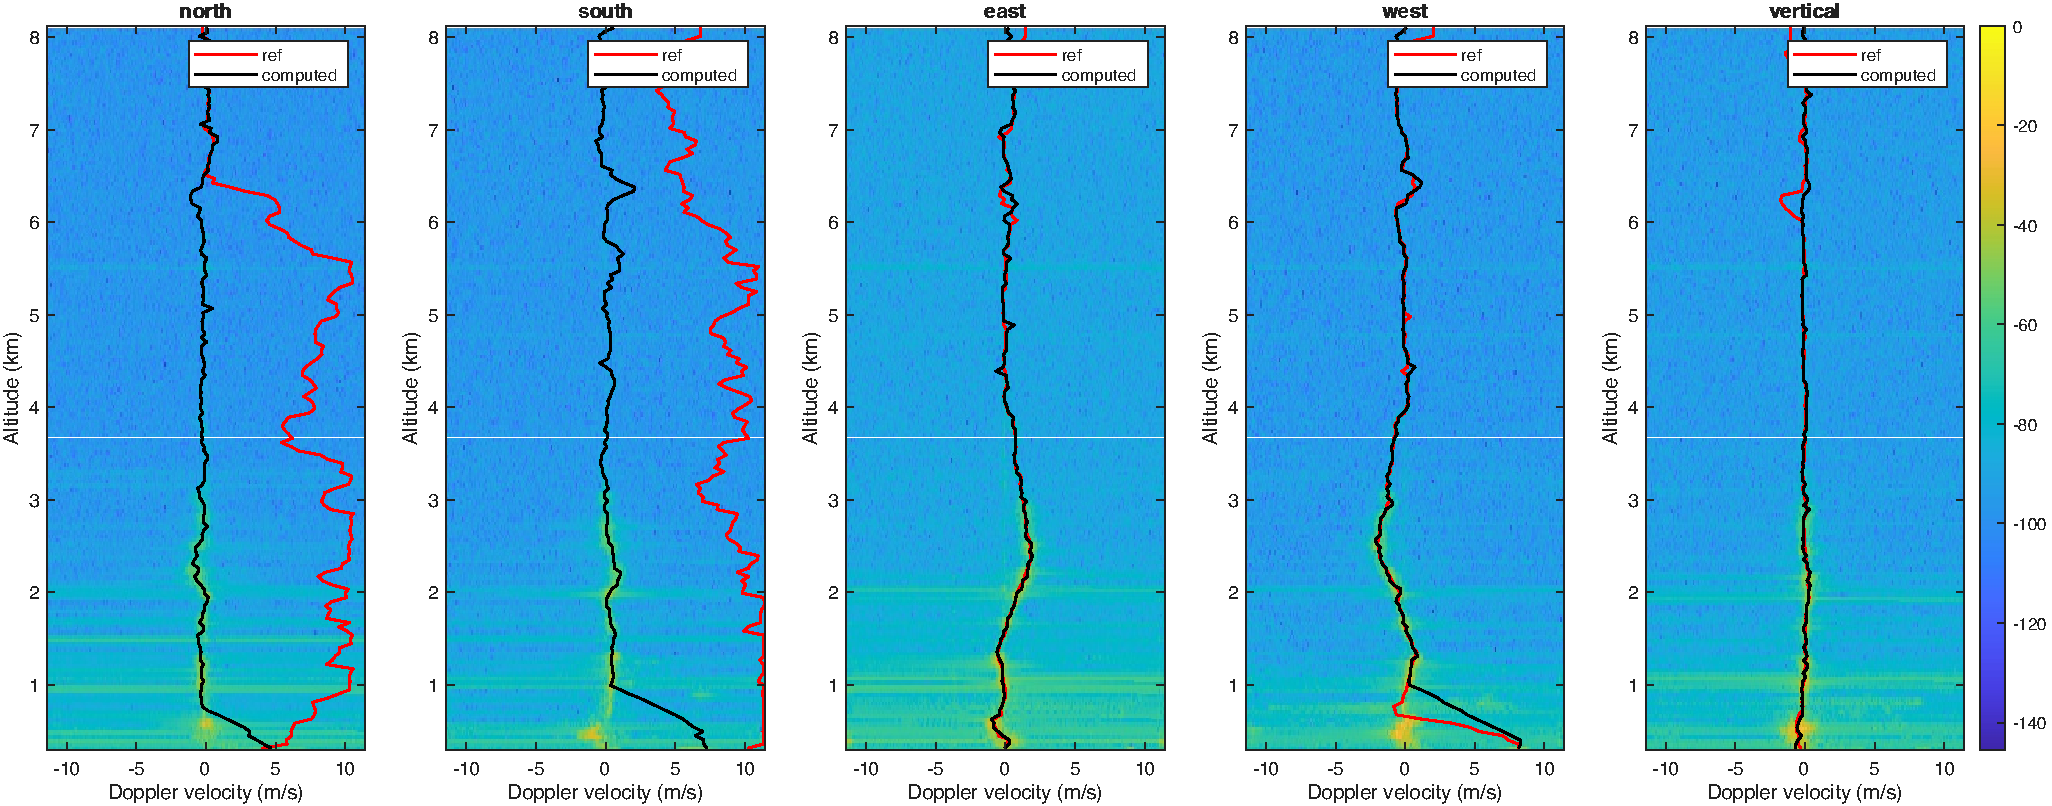
\includegraphics[width= \linewidth]{dp-obs54.pdf}
    \caption{\small Case where Data Pattern's algorithm fell short, moments computed by MCCF}
\end{figure}
\end{frame}



\section*{Conclusion}
\begin{frame}{Conclusion }
\small
\begin{itemize}
    \item Studied MCCF and IME for Doppler spectral peak and
    moment estimation using ST radar data.

    \item Examined two hybrid approaches combining mutual
    convolution with IME peak-selection and profile-tracing stages.

    \item The methods address challenges such as low SNR and
    unwanted spectral components.

    \item Methods were evaluated with various sources.
\end{itemize}
\end{frame}
\section{Future Scope}
\begin{frame}{Future Scope}
\begin{itemize}
    \item Wavelet-based denoising: Improve weak Doppler peak detection under low-SNR conditions.
    \item  ML-Based Peak Detection: Improve atmospheric echo identification in multi-peak spectra.
    \item  Making synthesised radar data more realistic by adding more features
    \item Distinguish rain echoes from clear-air atmospheric echoes in Doppler spectra to improve the reliability of wind-velocity estimation
    \item Can be used to fill gaps between observations in the lower atmosphere while the experiment is being conducted at higher altitudes
    \item Use synthetic data to train reinforcement learning-based algorithms for estimating wind profiles.
\end{itemize}
\end{frame}



    

\section*{References}
\begin{frame}[allowframebreaks]{References}
\begin{thebibliography}{6}
\bibitem{1}
Z. Tan, G. Yang, S. Wang, L. Wang, Y. Fan, R. Wang, and
Y. Luo, ``Wind Profile Estimation for K-Band Doppler Radar
Based on Mutual Convolution Cost Function Method,''
\textit{IEEE Sensors Journal}, vol. 24, no. 15,
pp. 24044--24053, Aug. 2024.
doi: 10.1109/JSEN.2024.3405665.

 

\bibitem{2}
Y. Li, R. Wang, Y. Luo, H. Li, and G. Yang,
``Improved Moments Estimation for Ground-Based K-Band
Doppler Radar Using Cost Function Method,''
\textit{IEEE Access}, vol. 10, pp. 32049--32059, 2022.
doi: 10.1109/ACCESS.2022.3159690.

\end{thebibliography}

\end{frame}
\section{}
\begin{frame}{}
    \centering
    \huge{\textbf{THANK YOU}}
\end{frame}

\end{document}